\chapter{Aprendizaje automático y Redes Neuronales}

En este capítulo trataremos los principales conocimientos de Aprendizaje Automático como su clasificación y importancia dentro del campo de la inteligencia artificial, además exploraremos algunos modelos importantes. 
En este seminario se dará énfasis en los algoritmos de clasificación. Luego nos enfocaremos en las redes neuronales para tratar más a fondo los problemas de clasificación.

\section{Aprendizaje Automático}
Machine Learning o Aprendizaje Automático es una rama de la inteligencia artificial que empezó a cobrar importancia en los años 80's. En esta rama se diseñan sistemas que aprenden a identificar patrones en un conjunto de datos. A medida que se realiza este aprendizaje, la máquina podrá ser capaz de realizar una predicción o tomar decisiones sin haber estado programada explícitamente para realizar esta tarea.


El Aprendizaje Automático se puede clasificar en 3 tipos: Supervisado, No supervisado, Aprendizaje con refuerzo.\cite{WEBSITE:2}
\subsection{Aprendizaje Supervizado}
Este tipo de aprendizaje  toma un conjunto de datos etiquetados, es decir datos cuyos resultados o clases son conocidos, estos datos serán usados como entrada al sistema. Primero se entrena el modelo con los datos de entrada y luego se trata de predecir  una salida de acuerdo a las etiquetas definidas.

 \textquotedblleft El aprendizaje supervisado trata de modelar la relación entre el resultado de la predicción y características de las entradas de manera que se puede predecir nuevos valores para un nuevo conjunto de datos \textquotedblright \cite{WEBSITE:1}
\subsection*{Tipos de problemas}
Dentro del aprendizaje supervisado podemos dividir los problemas en 2 tipos:
\subsubsection*{Problemas de Regresión Lineal}
Los problemas de regresión lineal son muy conocidos en el ámbito de Aprendizaje Automático y la estadística.
\subsubsection*{Problemas de Clasificación}
\textquotedblleft En este tipo de problemas se predice una respuesta del tipo categórica de manera que se puedan separar los datos mediante clases. \textquotedblright \cite{WEBSITE:2}

\textquotedblleft El objetivo de los problemas de clasificación es asignar resultados en categorías discretas en lugar de estimar valores continuos \textquotedblright \cite{WEBSITE:1}.\\
Un ejemplo de su uso son las tareas de reconocimiento de imágenes.

\begin{figure}[H]
	\centering
	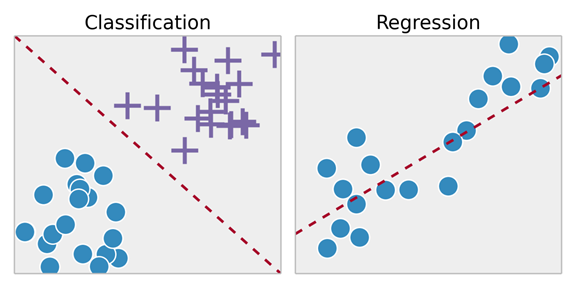
\includegraphics[width=0.9\textwidth]{Figures/regreclas.png}
	\caption{Regresión y clasificación \\ Fuente:  \href{https://medium.com/deep-math-machine-learning-ai/different-types-of-machine-learning-and-their-types-34760b9128a2}{\textit{https://medium.com/}}}
	\label{Regresion}
\end{figure} 

\subsubsection*{Algoritmos de Aprendizaje Supervisado}
\subsubsection*{Regresión Lineal}
\textquotedblleft El algoritmo de regresión lineal asume que existe una relación entre las variables de entrada $x=(x_{1},...,x_{n})$ y una salida simple $y$.  Cuando se tiene solo una variable simple $x$ el método se conoce como \textit{simple linear regression} y cuando se tienen múltiples entradas se le conoce como \textit{multiple linear regression}.  \textquotedblright \cite{WEBSITE:3} .Es comúnmente usado para estimar valores reales en base a variables continuas. La figura 3.2 muestra una regresión lineal simple.
\begin{equation}
\label{Simple learning regression}
y=b_{0}+b_{1}*x_{1}+b_{2}*x_{2}+.....+b_{n}*x_{n}
\end{equation} 
En esta ecuación:
\begin{itemize}
	\item $y$    : Variable dependiente
	\item $x_{i}$: Variable independiente i
	\item $b_{0}$: Intercepción
	\item $b_{1}$: Coeficiente para la primera característica
	\item $b_{n}$: Coeficiente para la primera característica
	
\end{itemize}
El objetivo del algoritmo de regresión lineal es obtener valores adecuados para los $b_{i}$  de manera que se reduzca la siguiente función de costo.
 \begin{equation}
 \label{eq:T3}
 \begin{aligned}
 J&=\frac{1}{n} \sum_{i=1}^{n}(pred_{i}-y_{i})^2
 \end{aligned}
 \end{equation}


\begin{itemize}
	\item $pred_{i}$: Predicción de la i-ésima variable
	\item $y_{i}$   : Valor real asociado a la i-ésima variable
	\item $n$       : Número de datos para el entrenamiento
	
\end{itemize}
Un método importante es la gradiente de descenso que se usa para actualizar valores de los $b_{i}$ de manera que se reduzca la función de costo $J$ de la ecuación 3.2. La figura 3.2 Nos muestra un conjunto de datos y la aplicación de la regresión lineal en estos.
\begin{figure}[H]
	\centering
	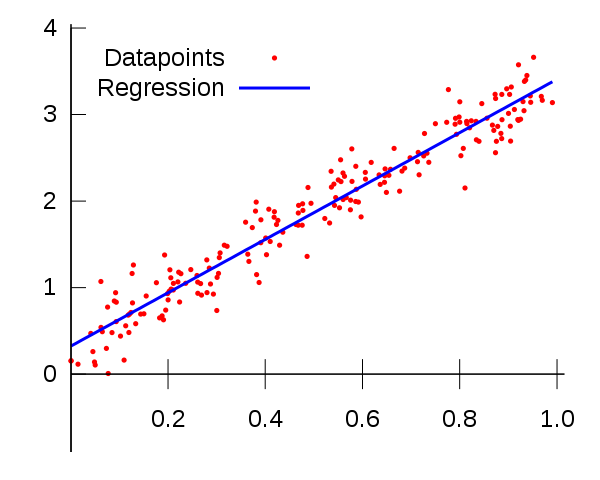
\includegraphics[width=0.9\textwidth]{Figures/Linear.png}
	\caption{Regresión Lineal \\ Fuente:  \href{https://www.forexmt4indicators.com/linear-regression-mt4-indicator/}{\textit{www.forexmt4indicators.com/}}}
	\label{Regresión Lineal}
\end{figure} 

\subsubsection*{Regresión Logística}
A diferencia de la Regresión Lineal, la Regresión Logística es usado para predecir el resultado de un variable de tipo categórica es decir variables que pueden ser descritas por un número finito de categorías.

 La regresión Logística es usado para problemas de clasificación lo cual realiza mediante la predicción de que una salida $Y$ dicótoma, es decir,que solo tenga 2 posibles valores.
 la regresión produce una curva, la cual genera valores entre 0 y 1.
 \textquotedblleft Matemáticamente podemos ver como que las salidas están modeladas como una combinación de los predictores lineales.\textquotedblright \cite{WEBSITE:6}
 \begin{equation}
 \label{eq:t}
 \begin{aligned}
 odds &= p/ (1-p)\\ 
 ln(odds) &= ln(p/(1-p))\\      
 logit(p) &= ln(p/(1-p)) = b_{0}+b_{1}X_{1}+b_{2}X_{2}+b_{3}X_{3}....+b_{k}X_{k}
 \end{aligned}
 \end{equation}
 %\end{equation} 
 
 \begin{itemize}
 	\item p : probabilidad de presencia de una característica de interés.
 	\item odds: probabilidad de éxito.
 	\item logit: función logit
 \end{itemize}
 
 Despejando p de las ecuaciones anteriores de 3.2 podemos obtener que:
  \begin{equation}
  \label{eq:t1}
  \begin{aligned}
  p&=\frac{1}{1+e^{b_{0}+b_{1}X_{1}+b_{2}X_{2}+b_{3}X_{3}....+b_{k}X_{k}}} \\
  Y_{pre}&=\frac{1}{1+e^{f(X)}}
  \end{aligned}
  \end{equation}
 En la ecuación 3.3, $Y$ define la función logística que se muestra en la figura 3.3. Esta también se puede conocer como la función sigmoidal en el perceptron.
 El algoritmo usa SGD para hallar los valores adecuados de $b_{i}$ de manera que el $erro=Y_{pre}- Y$ sea mínimo.
 El valor de la predicción es 1 si $Y_{pred}>0.5$ y 0 en caso contrario. De esta forma se determina el objeto con características $X$ si pertenece o no a una clase.
 
 \begin{figure}[H]
 	\centering
 	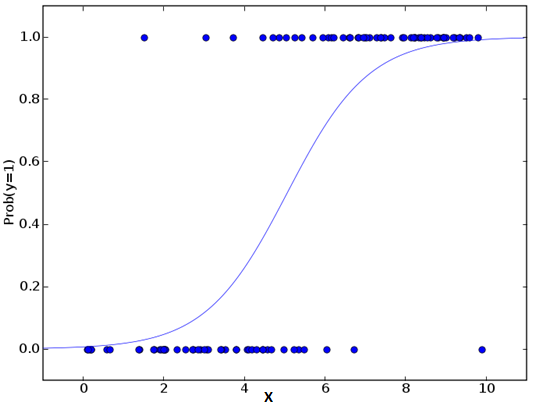
\includegraphics[width=0.9\textwidth]{Figures/logistic.png}
 	\caption{Regresión Logística \\ Fuente:  \href{https://www.analyticsvidhya.com/blog/2017/09/common-machine-learning-algorithms/}{\textit{www.analyticsvidhya.com}}}
 	\label{Regresión Logistica}
 \end{figure} 
\subsubsection*{Nearest Neighbor}
Es un algoritmo de clasificación que almacena los conjuntos de entrenamiento de manera que dado un nuevo ejemplo $x$ lo clasifica buscando la distancia  más cercana a un ejemplo de entrenamiento $(x_{i},y_{i})$ de manera que identifica la clase $y=y_{i}$ a la que corresponde.

 Comúnmente se usa el algoritmo k-nn para clasificar una entrada $x$ en los k más cercanos conjuntos de entrenamiento y asigna el objeto a la clase de más frecuencia.

  \begin{equation}
  \label{eq:t12}
  \begin{aligned}
  x^i=(x_{1}^i,x_{2}^i,.... ,x_{n}^i)\\
  d_{E}(x^i,x^j)
  \end{aligned}
  \end{equation}
\begin{itemize}
	\item $x^i$: objeto con n características.
	
\end{itemize}

Definimos $d_{E}$ como la función distancia entre los vectores  $x_{i}$ y $y_{i}$ .\\ Esta función distancia puede clasificarse en:

  \begin{itemize}

  \item Distancia Euclideana:    $(\sum_{i=1}^{k}(x_{i} - y_{i})^2)^\frac{1}{2}$
  \item Distancia Manhattan:     $\sum_{i=1}^{k}|x_{i} - y_{i})|  $
  \item Distancia Minkowski:     $(\sum_{i=1}^{k}(|x_{i} - y_{i}|)^p)\frac{1}{p}$
  \end{itemize}
Los 3 definiciones anteriores de distancia son usadas en variables continuas.  Para el caso de las variables categóricas se deberá usar la distancia de Hamming cuya definición se muestra en la ecuación 3.6


  \begin{equation}
  \label{eq:t6}
  \begin{aligned}
  	D_{H}&=\sum_{i=1}^{k}|x_{i} - y_{i})|\\
  	x&=y \Longrightarrow D=0\\
  	x&\neq y \Longrightarrow D=1
  \end{aligned}
  \end{equation}
  	
\textquotedblleft La elección de un valor óptimo k se logra mejor por la inspección de los datos. En general un valor grande de k es más preciso, ya que reduce el ruido pero no hay garantías de que sea un valor correcto, una mejor manera de calcular el valor de $k$ es mediante el uso de la validación cruzada.
\textquotedblright \cite{WEBSITE:7}

En la figurar 3.4 muestra el algoritmo de k-nn dado un nuevo ejemplo(círculo verde) este será clasificado de acuerdo al \textit{k} seleccionado. Para $k=1$ el nuevo ejemplo será clasificado en la clase 1 y $k=3$ será clasificado en la clase 2.
 \begin{figure}[H]
 	\centering
 	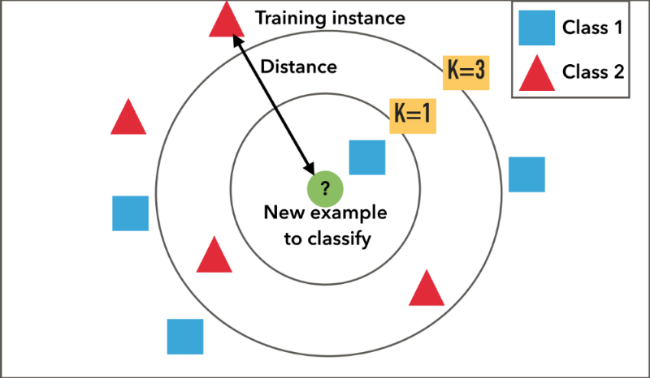
\includegraphics[width=0.7\textwidth]{Figures/knn.png}
 	\caption{knn \\ Fuente:  \href{https://medium.com/@adi.bronshtein/a-quick-introduction-to-k-nearest-neighbors-algorithm-62214cea29c7}{\textit{www.medium.com/}}}
 	\label{knn}
 \end{figure} 
\subsubsection*{Máquinas de soporte Vectorial(SVM)}
Las Maquinas de soporte vectorial fueron creadas por Vladimir Vapnik y constituyen un método para realizar tareas de clasificación y regresión.\\ Las SVM usan el concepto de planos de decisión. Un plano de decisión separa un conjunto de objetos que tienes diferentes etiquetas de clases. Las SVM no están restringidas a los problemas lineales debido a las \textit{funciones Kernel.}
\textbf{Funciones Kernels}\\
Las SVM pueden tener distintos tipos de kernels que tienen como objetivo tomar la data y transformarla. Algunas funciones kernels conocidas:
\begin{itemize}
	\item Lineal: $\ker(x_{i},x_{j})= x_{i} \cdot x_{j}$
	\item Polinomial: $\ker(x_{i},x_{j})= ( \gamma x_{i} \cdot x_{j}+C)^d$
	\item Radial: $\ker(x_{i},x_{j})= e^{(\gamma |x_{i} - x_{j}|)}$
	\item Sigmoidal: $\ker(x_{i},x_{j})= \tanh ( \gamma x_{i} \cdot x_{j}+C)$
\end{itemize}
En la figura 3.5 muestra el efecto de las funciones kernels en un conjunto de datos para que este sea linealmente separable sin necesidad de construir curvas complejas.\\
\begin{figure}[H]
	\centering
	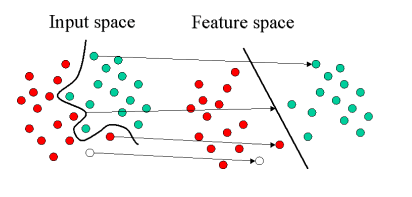
\includegraphics[width=0.9\textwidth]{Figures/kernel.png}
	\caption{transformación con la función kernel \\ Fuente:  \href{http://www.statsoft.com/Textbook/Support-Vector-Machines}{\textit{www.statsoft.com}}}
	\label{transformación con la función kernel}
\end{figure} 

Podemos dividir SVM en 2 categoríasas:\\
\textbf{Super Vector Classificacion}\\
Los SVC realizan la tarea de clasificación encontrando un hiperplano que maximicé el margen entre 2 clases.Los vectores que definen el hiperplano son llamados \textit{support vector}.\\ Para la clasificación es necesaria mapear los datos a un espacio de características de mayor dimensión donde resulte más fácil la separación lineal.  La imagen de la Figura 3.5 muestra de manera gráfica que cambio de espacio nos permite separar clases de manera más sencilla.\\ \\
\textbf{Super Vector Regression}\\
SVR trata de mapear los datos de entrenamiento $x \in X$ , a un espacio de mayor dimensión mediante una mapeo no lineal $ \varphi : X \to F$ .\\
Las SVR son parecidas a las máquinas de soporte Vectorial para la clasificación pero con la diferencia de que la salida es un número real que es difícil de predecir con la información que se posee además de que tiene infinitas posibilidades. Para los problemas de regresión se usan los kernels Radial y polinomial. La figura 3.6 muestra un ejemplo de problema de regresión para un caso no lineal, mediante la mapeo $ \varphi $ se cambia el espacio.

\begin{itemize}
	\item caso lineal:     $y=\sum_{i=1}^{N}(\alpha_{i}  -\alpha_{i}^*)\langle x_{i},x\rangle +b$
	\item caso no lineal:  $ y=\sum_{i=1}^{N}(\alpha_{i}  -\alpha_{i}^*)\ker(x_{i},x) +b$
\end{itemize}

\begin{figure}[H]
	\centering
	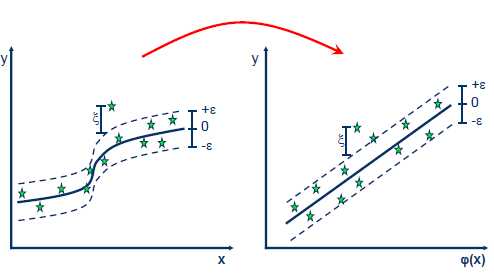
\includegraphics[width=0.7\textwidth]{Figures/SVR.png}
	\caption{transformación para un problema de regresión \\ Fuente:  \href{http://www.saedsayad.com/support_vector_machine_reg.htm}{\textit{www.saedsayad.com}}}
	\label{transformacion}
\end{figure} 

\subsubsection*{Naive Bayes}
Esta basado en el Teorema de Bayes donde se asume la independencia entre los predictores.\textquotedblleft El modelo Naive Bayes es fácil de construir, debido a que no tiene la necesidad de estimar los parámetros iterativamente por lo cual es particularmente útil para un gran conjunto de datos \textquotedblright \cite{WEBSITE:8}.\\
Como la  técnica de clasificación se basa en el Teorema de Bayes supone que cada característica de una clase no esta relacionada con otras características.\\ Podemos ilustrar mejor lo dicho mediante el siguiente ejemplo  \textquotedblleft Una fruta puede considerarse una manzana si es roja, redonda y de aproximadamente 3 pulgadas de diámetro. Incluso si estas características dependen unas de otras o de la existencia de otras características, todas estas propiedades contribuyen de forma independiente a la probabilidad de que esta fruta sea una manzana y es por eso que se la conoce como \textbf{Naives}  \textquotedblright \cite{WEBSITE:4}


\begin{equation}
  \label{eq:naives}
  \begin{aligned}
  P(c|x)&=\frac{P(x|c)P(c)}{P(x)}\\
  P(c|X)&=P(x_{1}|c)\times P(x_{2}|c)\times ... \times P(x_{n}|c)\times P(c)
  \end{aligned}
\end{equation}

\begin{itemize}
	\item $P(c|x):$ Probabilidad condicional de una clase(target) dado un predictor(atributo)
	\item $P(c):$ Probabilidad de la clase
	\item $P(x|c):$Probabilidad condicional de la clase dada por el predictor.
	\item $P(x):$ Probabilidad del predictor.
	
\end{itemize}

\subsubsection*{Arboles de decisión}
Los arboles de decisión son modelos usados para tareas de regresión y clasificación, estos utiliza la estructura de un árbol. La idea se basa en dividir el conjunto de datos en subconjuntos cada vez más pequeños que a su vez desarrolla un árbol de decisión. El resultado final será un árbol con nodos de decisión y nodos hojas.\\
Los nodos de decisión tienen 2 o más ramas y los nodos hojas representa una clasificación o decisión. La raíz corresponde al mejor predictor. Un árbol de decisión puede ser usado para manejar datos categóricos o numéricos.\\

\textbf{Árbol de decisión para clasificación}.\\
El algoritmo principal para construir un árbol de decisión es el ID3 que fue desarrollado por J. R. Quinlan.\\ \textquotedblleft ID3 realiza una algoritmo greeady para realizar un búsqueda de arriba hacia abajo a través del espacio de posibles ramas . ID3 usa entropía e información ganada para construir el árbol de decisión \textquotedblright.\\ A diferencia de Naives Bayes, en un árbol de decisión es importante asumir la dependencia de los predictores.\\
\begin{itemize}
	\item \textbf{Entropía}: Para el algoritmo ID3 es importante tener la entropía para calcular la homogeneidad de la muestra.
	\item \textbf{Información ganada}: se basa en la disminución de la entropía después que un conjunto de datos se divide en atributos.
\end{itemize}

\textbf{Árbol de decisión para regresión}.\\
Al igual que el caso de clasificación, se usa el algoritmo ID3 con la diferencia que se usa la información ganada por la desviación estándar de reducción. Este tipo de desviación se basa en la disminución de la desviación estándar cuando el conjunto de datos se divide en un atributo.

\subsection{Aprendizaje No Supervisado}
Mientras que el aprendizaje supervisado aprende en base a un conjunto de datos de entrenamiento que contienen respuestas o etiquetas correctas. En el aprendizaje no supervisado los datos de entrenamiento no poseen ninguno tipo de etiqueta, por lo tanto los sistemas deben de interpretar los datos por si mismos.
El aprendizaje no supervisado es usado principalmente para el reconocimiento de patrones y modelado descriptivo.
A continuación discutiremos algunos algoritmos del Aprendizaje No Supervisado.
\subsubsection*{Clustering}
Clustering se refiere a agrupar objetos con características similares, es decir buscar la relación entre ellos sin necesidad de que exista un conocimiento a priori de esos grupos.
\begin{figure}[H]
	\centering
	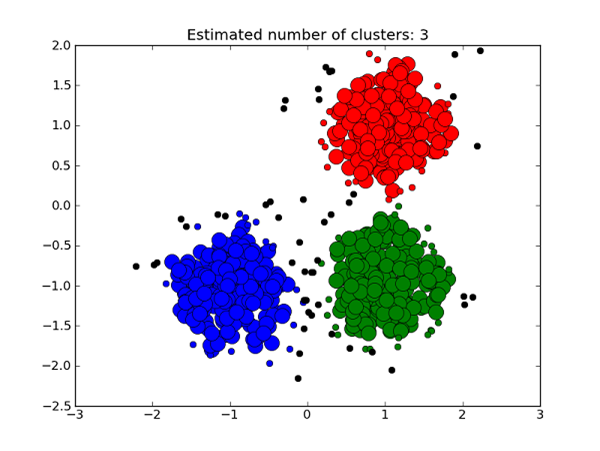
\includegraphics[width=0.5\textwidth]{Figures/clustering.png}
	\caption{Clustering \\ Fuente:  \href{https://medium.com/deep-math-machine-learning-ai/different-types-of-machine-learning-and-their-types-34760b9128a2}{\textit{https://medium.com/}}}
	\label{Clustering}
\end{figure} 
\subsubsection*{K-means Clustering}
El algoritmo realiza la partición de  $N$ objetos en $k$ clusters en los cuales cada objeto pertenece al cluster que posee la media más cercana. Este método produce $k$ clústeres con la mayor distinción posible. El k adecuado no se conoce a priori por lo cual debe calcularse a partir de datos. El objetivo de k-means es minimizar la función de error al cuadrado mostrada en la ecuación 3.8.

\begin{equation}
  \label{eq:clustering}
  \begin{aligned}
  J&= \sum_{j=1}^{k} \sum_{i=1}^{n}\parallel x_{i}^j - c_{j}\parallel ^2
  \end{aligned}
\end{equation}

\begin{itemize}
	\item $J$: Función de error cuadrado.
	\item $k:$ Número de cluster.
	\item $n:$ Número de casos.
	\item $x_{i}^j:$ Objeto i
	\item $c_{j}:$ Centroide del cluster j
\end{itemize}
%%% añadir algoritmo
\begin{figure}[H]
	\centering
	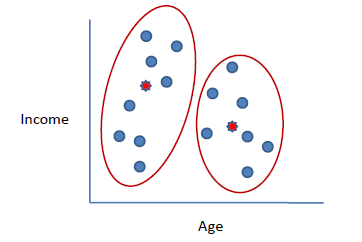
\includegraphics[width=0.7\textwidth]{Figures/kmeans.png}
	\caption{k means clustering\\ Fuente:  \href{http://www.saedsayad.com/clustering_kmeans.htm}{\textit{www.saedsayad.com}}}
	\label{kmeans}
\end{figure} 


\subsection{Aprendizaje por refuerzo}
Este tipo de aprendizaje fue inspirado por la psicología conductista, este busca determinar que tipo de acciones tomar en un entorno dado. \textquotedblleft El objetivo del método es recopilar la interacción con el entorno para tomar acciones que maximicen el beneficio o minimicen el riesgo. \textquotedblright \cite{WEBSITE:1}

\begin{figure}[H]
\begin{center}
	\smartdiagramset{circular distance=4cm,
		font=\large,
		text width=2.5cm,
		module minimum width=2.5cm,
		module minimum height=1.5cm,
		arrow tip=to}
	\smartdiagram[circular diagram]{Agente,Accion, entorno,refuerzo}
	
\end{center}
\caption{Esquema de aprendizaje por refuerzo \\ Fuente:  \textit{Fuente Propia}}
\label{refuerzo}
\end{figure}

\section{Redes Neuronales}
\subsection{Neuronas}
En la biología, la neurona es conocida como la unidad fundamental del cerebro humano, el cual está compuesto por millones de neuronas interconectadas entre si(sinapsis). El trabajo de las neuronas consiste en recibir información, procesarla y enviarla a otras células.\\ Este modelo fue copiado en 1943 por Warren S. McCulloch y Walter H. Pitts para poder diseñar un neurona artificial que es análoga a las neuronas del cerebro humano, la neurona artificial tomará una cantidad n de entradas $x_{1}, x_{2}, x_{3}, .. , x_{n}$ estas entradas serán multiplicadas por pesos $w_{1}, w_{2}, w_{3}, .. , w_{n}$ además se puede añadir una constante que llamaremos bias($b$) para producir un salida.

La entrada a la neurona será la suma total de los productos z=  $\sum_{i=1}^{n}{ w_{i}x_{i}}+b$ , el valor de z , esta se evaluará con una función f de tal forma que nuestra salida será $y=f(z)$.\\ En la ecuación 3.9 observamos la misma salida expresada en forma vectorial para nuestros vectores  $x = [x_{1}  x_{2}  x_{3}  ...  x_{n}]$ y $w = [w_{1}  w_{2}  w_{3}  ...  w_{n}]$



\begin{equation}
\label{forma vectorial}
\begin{aligned}
y&=f(x\cdot w+b)
\end{aligned}
\end{equation}
\subsubsection{Funciones de Activación}
La función $f$ anteriormente mencionada es una función no lineal, conocida como función de activación.\\ La tarea principal de la función de activación es introducir no linealidad a la salida de una neurona. Esto es importante debido a que la vida real no trabajamos con datos no lineal y de esta forma la neurona puede aprender representaciones no lineales.\\ Entre funciones de activación tenemos algunas comúnmente usada como:
\begin{itemize}
	\item \textbf{Sigmoid}: Toma un valor real, y lo transforma en una valor en el rango de 0 a 1.\\
	$ \sigma (x) = \frac{1}{1+e^{-x}}$
	\item \textbf{tanh}: Toma por entrada un valor real y lo transfroma a un número en le rango de -1 a 1.\\
	$\tanh (x)=\frac{2}{1+e^{-x}} -1$
	\item \textbf{ReLu}: o Unidad lineal rectificada es una función que para valores menores que 0 asigna 0 y para valores mayores 
	\[   
	f(x) = 
	\begin{cases}
	\text{0} &\quad x<0\\
	\text{x} &\quad x\geq0\\

	\end{cases}
	\]
\end{itemize}
\begin{figure}[H]
	\centering
	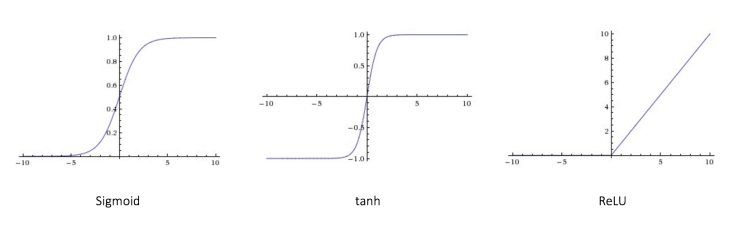
\includegraphics[width=0.9\textwidth]{Figures/factivacion.png}
	\caption{Funciones de activación \\ Fuente:  \href{https://ujjwalkarn.me/2016/08/09/quick-intro-neural-networks/}{\textit{https://ujjwalkarn.me}}}
	\label{activacion}
\end{figure} 

\subsection{Redes Neuronales Artificiales}
Las redes neuronales artificiales(ANN)toman de ejemplo la arquitectura del cerebro como inspiración para la construcción de sistemas inteligente. Actualmente son la base para el desarrollo de la inteligencia artificial.\\
Una red neuronal está constituida por las uniones de neuronas.\\
En la figura 3.10 podemos ver la comparación entre una neurona biológica y un artificial etiquetadas con A y B respectivamente. Además observamos que las redes neuronales artificiales (etiqueta D) imitan el la unión biológicas de las neuronas o sinapsis(Etiqueta C).

\begin{figure}[H]
	\centering
	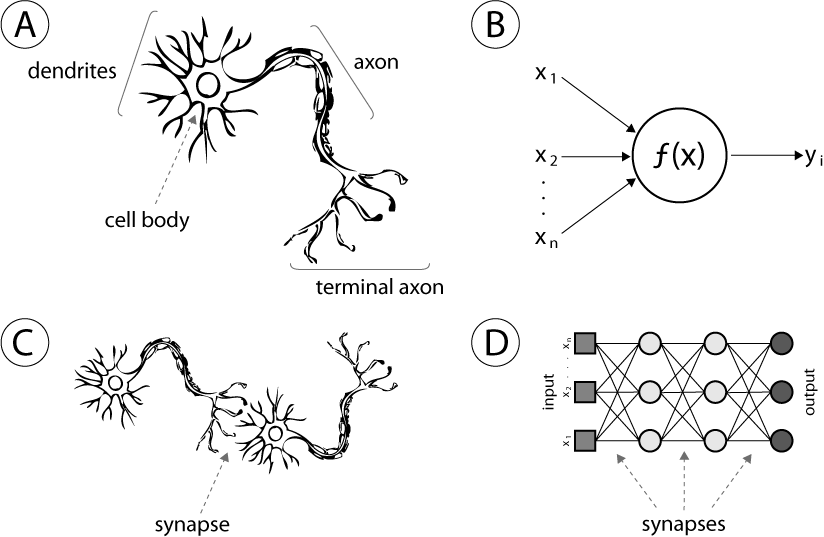
\includegraphics[width=0.8\textwidth]{Figures/ANN.png}
	\caption{Redes neuronales biológicas y artificiales \\ Fuente:  \href{https://medium.com/@ivanliljeqvist/the-essence-of-artificial-neural-networks-5de300c995d6}{\textit{https://medium.com}}}
	\label{neuronas}
\end{figure} 
\subsubsection{Redes Neuronales Prealimentadas}
Estás redes fueron de las primeras y más simples de los tipos de redes neuronales que fueron desarrolladas. Contienen múltiples neuronas (nodos) ordenadas en capas de modo que los nodos en capas adyacentes se conectan. Cada una de estas conexiones poseen un peso asociado a dicha conexión.\\
En la figura 3.12 mostramos el esquema de Redes prealimentadas con sus distintas capas(layer).
\begin{figure}[H]
	\centering
	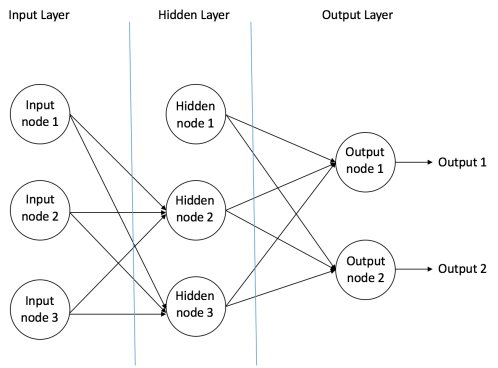
\includegraphics[width=0.9\textwidth]{Figures/esquemaff.png}
	\caption{Esquema de Redes Neuronales Prealimentadas \\ Fuente:  \href{https://ujjwalkarn.me/2016/08/09/quick-intro-neural-networks/}{\textit{https://ujjwalkarn.me}}}
	\label{neuronasredes}
\end{figure} 
\begin{itemize}
	\item \textbf{Nodo de entrada(Input Node):} Proveen información a la red. En conjunto representan la capa de entrada, ningún calculo es realizado en esta capa solo se transfiere la información a la capa oculta.
	\item \textbf{Nodo Oculto(Hidden Node):} El trabajo de los nodos ocultos es calcular y transferir la información hacia a el nodo de salida. Una Red prealimentada tiene solo una capa de entrada y una salida pero puede tener múltiples capas ocultas.
	\item \textbf{Output Node:}Su tarea principal es realizar cálculos y transferir la información fuera de la red.
\end{itemize}
En las redes neuronales prealimentadas, la información solo se propaga en una dirección hacia adelante desde los nodos de entradas pasando por los nodos ocultos hacia los nodos de salida. No existen ciclos en este tipo de red.\\
Dentro de las redes neuronales prealimentadas tenemos algunos ejemplos:
\begin{itemize}
	\item \textbf{Perceptron Simple:} Es un red prealimentada simple que no posee capa oculta.Solo puede aprender de funciones lineales.
	\item \textbf{Perceptron Multicapas:} Esta red posee una o más capas ocultas. Este perceptron puede aprender de funciones no lineales.
	\item \textbf{Redes neuronales de convolución:} Este tipo de redes neuronal será explicada con más detalle en el capítulo 4 sección 1.
\end{itemize}
\subsubsection{Algoritmo de propagación hacia atrás}
La propagación hacia atrás trata de aprender de los errores, como ya hemos visto en el aprendizaje supervisado los conjuntos de entrenamiento se encuentran etiquetados. Por lo cual podemos saber cual es la salida esperada. \\
El algoritmos se aplica de la siguiente forma:

\begin{enumerate}
	\item Se toma un ejemplo y se asignan pesos aleatorios a todas las conexiones de la red. Luego por medio de las conexiones y funciones de activación se calcula la salida en las capas ocultas y de salida.
	\item Se calcula el error total y se propagan estos errores hacia atrás a través de la red y se calcula la gradiente, luego se usan métodos como gradientes de descenso para ajustar los pesos y reducir el error en la capa de salida. La técnica de gradiente de descenso será explicada con más detalle en el siguiente capítulo.
	\item Se repite el proceso con los otros ejemplos
\end{enumerate}
\begin{figure}[H]
	\centering
	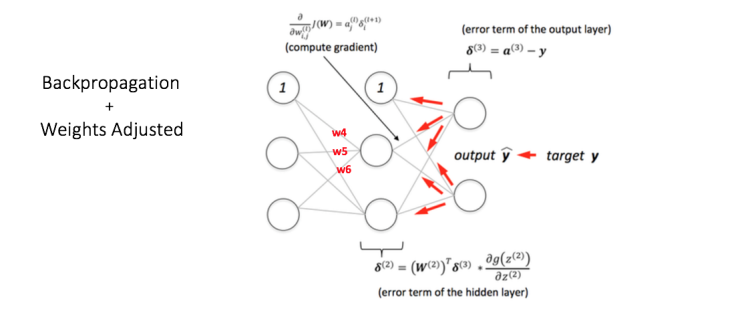
\includegraphics[width=0.9\textwidth]{Figures/backp.png}
	\caption{Propagación hacia atrás \\ Fuente:  \href{https://ujjwalkarn.me/2016/08/09/quick-intro-neural-networks/}{\textit{https://ujjwalkarn.me}}}
	\label{backpropagation}
\end{figure} 
\subsubsection{Conjunto de datos para una red neuronal}
Para alimentar nuestra red es importante tener información que le permita aprender. Esta información es llamada conjunto de datos o dataset, el cual nos permite entrenar a nuestra red y testearla.\\ Una tarea principal para construir nuestro modelo es separar este dataset en 3 categorías.
\begin{itemize}
	\item \textbf{Datos de entrenamiento:} Permite entrar nuestro modelo.
	\item \textbf{Datos de Validación:} Permite evaluar y actualizar los parámetros de entrenamiento
	\item \textbf{Datos de testeo:} Permite testear el funcionamiento del modelo al ingresar datos nuevos.
\end{itemize}
Con esta división es posible entrenar nuestra red y verificar su funcionamiento. La figura 3.14 nos muestra el esquema de la división de los datos.
\begin{figure}[H]
	\centering
	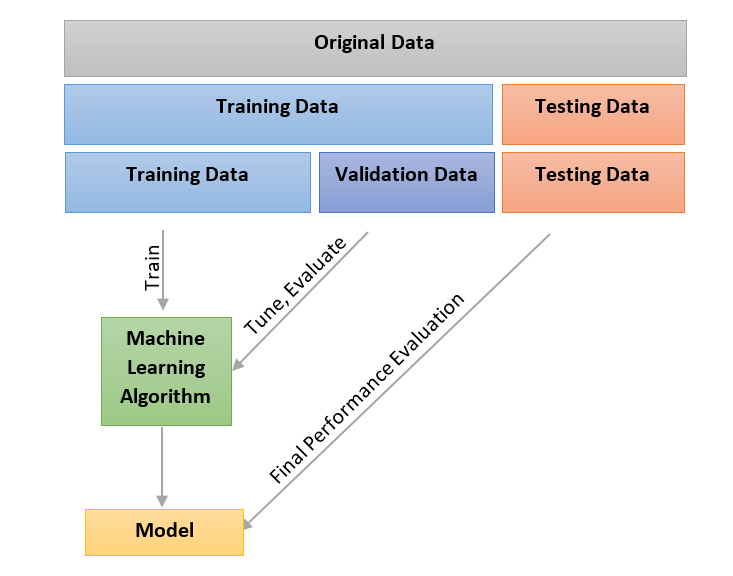
\includegraphics[width=0.9\textwidth]{Figures/validation.PNG}
	\caption{División del dataset \\ Fuente:  \href{http://magizbox.com/training/machinelearning/site/evaluation/}{\textit{http://magizbox.com}}}
	\label{validacion}
\end{figure} 




%%\subsubsection*{Características}
%%%
%%\begin{figure}[H]
%%\centering
%%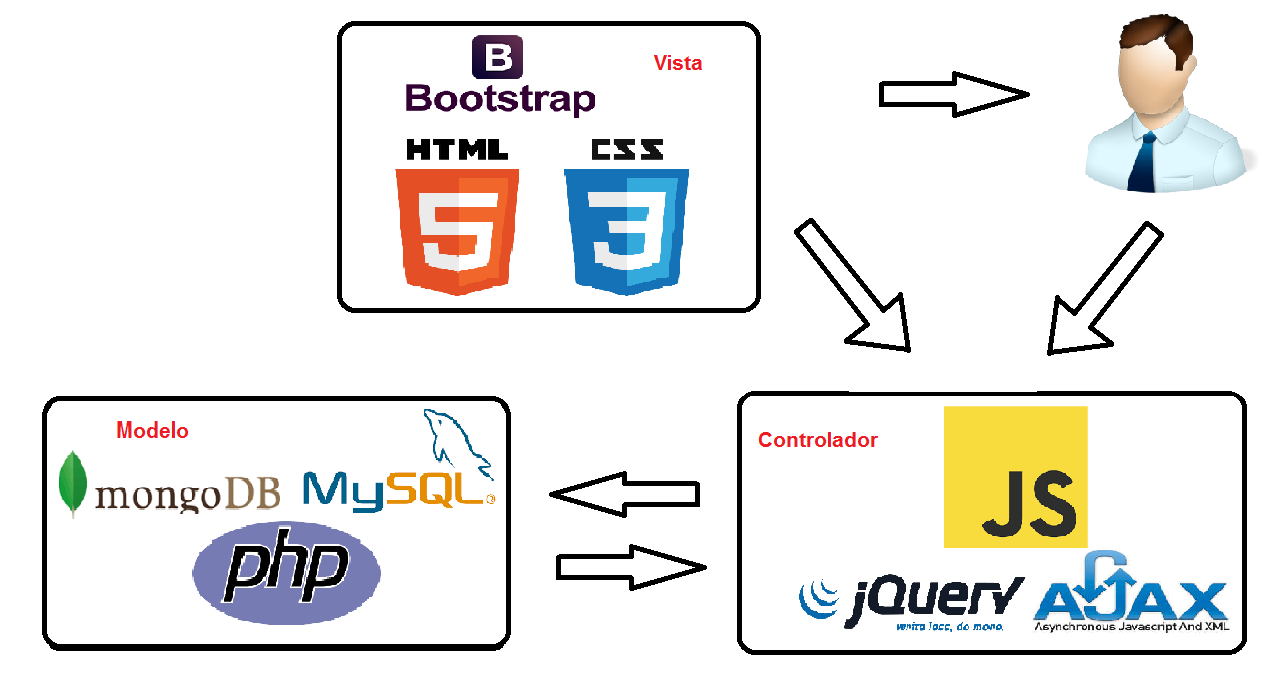
\includegraphics[width=0.9\textwidth]{Figures/mvc.png}
%%\caption{Modelo-Vista-Conrolador}
%%\label{MVC}
%%\end{figure}



\afterpage{\blankpage}